\documentclass[crop,border=7pt]{standalone}
\usepackage{tikz}
\usepackage{ifthen}
\usetikzlibrary{shapes.geometric}
\tikzset{
  hexagone/.style={
    draw, thick,
    fill=blue!20,
    shape=regular polygon,
    regular polygon sides=6,
    outer sep=0, inner sep=0,
    minimum size=1cm,
    %label={[red]center:#1}
  }
}
\begin{document}
  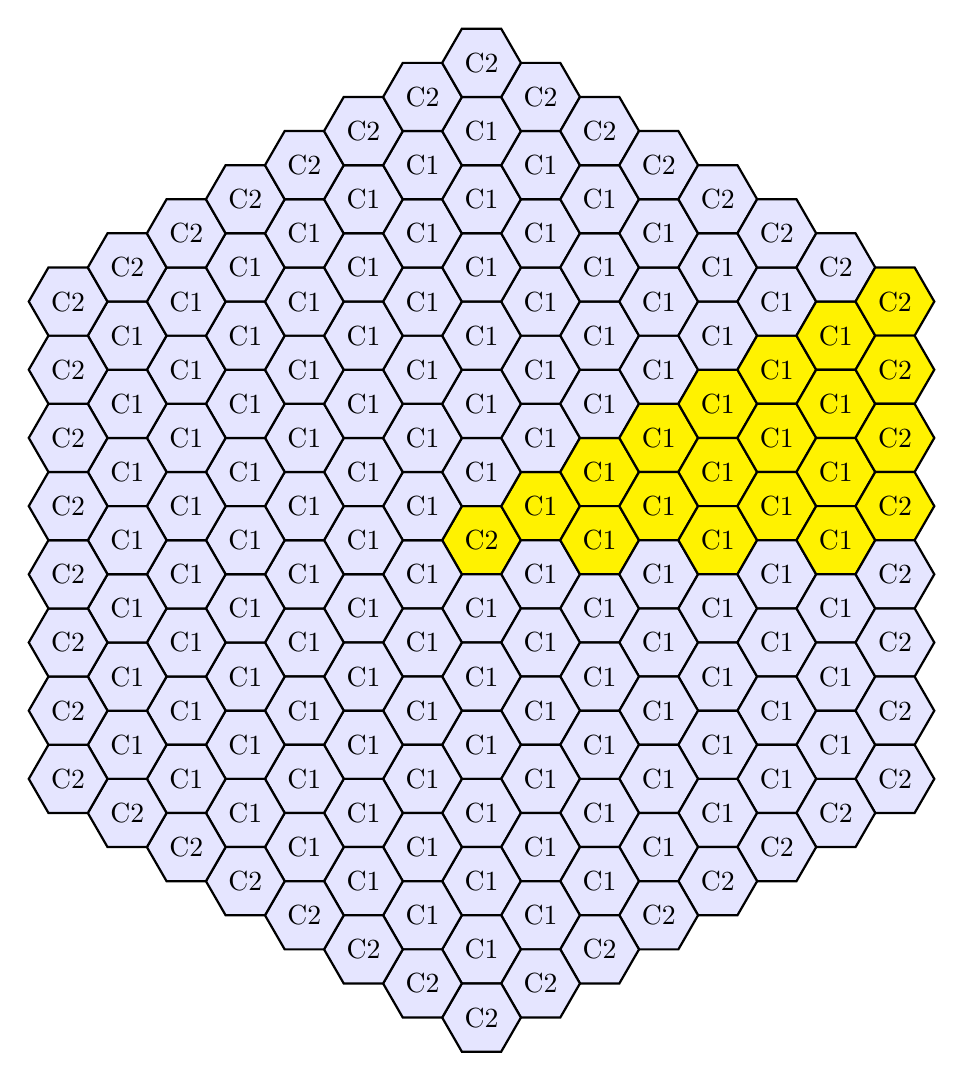
\begin{tikzpicture}
  %%%%%%%%%%%%%%%%%%%%%%%%%%
    \node[hexagone=0, fill=yellow, label={[black]center:C2} ] at (0,0){};
    \foreach \r in {1,...,6}
      \foreach \t in {0,...,5}
        \foreach[evaluate={\l=int(\r*(\r-1)*3+\r*\t+\u)}] \u in {1,...,\r}
        \ifthenelse{\l=1 \OR \l=8 \OR \l=9 \OR \l=21 \OR \l=22 \OR \l=40 \OR \l=41 \OR \l=42 \OR \l=65 \OR \l=66 \OR \l=67 \OR \l=96 \OR \l=97 \OR \l=98 \OR \l=99}{\def\mycolor{yellow}}{\def\mycolor{blue!10}}
          \scoped[rotate=-\t*60]
            \node[hexagone=\l, fill=\mycolor, label={[black]center:C1}] at (0+.75*\u,{0.43301270189*(2*\r-\u)}){};
            
            
            \foreach \r in {7,...,7}
      \foreach \t in {0,...,5}
        \foreach[evaluate={\l=int(\r*(\r-1)*3+\r*\t+\u)}] \u in {1,...,\r}
        \ifthenelse{\l=133 \OR \l=134 \OR \l=135 \OR \l=136}{\def\mycolor{yellow}}{\def\mycolor{blue!10}}
          \scoped[rotate=-\t*60]
            \node[hexagone=\l, fill=\mycolor, label={[black]center:C2}] at (0+.75*\u,{0.43301270189*(2*\r-\u)}){};
   
   
   
   
    %Legend
%         \node[anchor=east] at (-9,-6) (leg1) {$1$. PSU};
%         \node[below=1mm of leg1] (leg2) {$2$. Sputter Source};
%         \node[right=6mm of leg1,anchor=west] (leg8) {$8$. Pumps};

%%LEGEND
%\draw (7,5.5) rectangle (12,10);
%\matrix [below left] at (current bounding box.north east) {
%  \node [bluenode, label=right:\LARGE In-Pile Section] {}; \\  
%  \node [violetnode, label=right:\LARGE Safety Rod] {}; \\
%  \node [yellownode, label=right:\LARGE Inner MOX Fuel] {}; \\
%  \node [rednode, label=right:\LARGE Outer MOX Fuel ] {}; \\
%  \node [greennode, label=right:\LARGE Control Rod] {}; \\  
%  \node [graynode, label=right:\LARGE Dummy Section] {}; \\  
%};

  \end{tikzpicture}
\end{document}